\documentclass[11pt, a4paper, twoside, openright]{article} 

\usepackage{graphicx,color}
\usepackage{amssymb, amsmath, array, cite, float, url}



\begin{document}

% Example of title page for the projects carried out within DEDIS
% Copied from lasec 

% Simply include it in your mastex tex file: 
%        % Example of title page for the projects carried out within DEDIS
% Copied from lasec 

% Simply include it in your mastex tex file: 
%        % Example of title page for the projects carried out within DEDIS
% Copied from lasec 

% Simply include it in your mastex tex file: 
%        \input{cover}


% Updated October 2016


\newcommand{\logoepfl}[0]{
  \begin{center}
    
\includegraphics[width=4cm]{logo_epfl_coul.eps}
  \end{center}
  \vspace{0.3cm}
  \hrule
}
\newcommand{\project}[1]{
  \begin{center}
    \large{#1}
  \end{center}
  \vspace{1cm}
}
\newcommand{\department}[1]{
  \begin{center}
    \large{#1}
  \end{center}
}
\newcommand{\lab}[1]{
  \begin{center}
    \large{#1}
  \end{center}
}
\newcommand{\supervisor}[3]{
  \begin{center}
    \begin{normalsize}{
        \bf #1}\\#2\\#3
    \end{normalsize}
  \end{center}
}
\renewcommand{\author}[1]{
  \begin{center}
    \Large{#1}
  \end{center}
  \vspace{0.5cm}
}
\renewcommand{\title}[1]{
  \vspace{3cm}
  \begin{center}
    \huge{#1}
  \end{center}
  \vspace{1.7cm}
}
\renewcommand{\date}[2]{
  \begin{center}
    \normalsize{#1 #2}
  \end{center}
  \vspace{0.5cm}
}


\thispagestyle{empty}


% begin title page
  \logoepfl
  
  \title{WebAssembly Execution Environment for Dela
}
  
  \author{Maxime Sierro}
  \department{School of Computer and Communication Sciences}
  \lab{Decentralized and Distributed Systems lab}
  \project{Master Semester Project}
  
  \date{June}{2021}

  \begin{center}
    \begin{tabular}{cc}
      \begin{tabular}{p{4.0cm}}
        \supervisor{Responsible}{Prof. Bryan Ford}{EPFL / DEDIS}
      \end{tabular}&
      \begin{tabular}{p{4.0cm}}
        \supervisor{Supervisor}{Noémien Kocher}{EPFL / DEDIS}
      \end{tabular}
    \end{tabular}
  \end{center}

% end title page




% Updated October 2016


\newcommand{\logoepfl}[0]{
  \begin{center}
    
\includegraphics[width=4cm]{logo_epfl_coul.eps}
  \end{center}
  \vspace{0.3cm}
  \hrule
}
\newcommand{\project}[1]{
  \begin{center}
    \large{#1}
  \end{center}
  \vspace{1cm}
}
\newcommand{\department}[1]{
  \begin{center}
    \large{#1}
  \end{center}
}
\newcommand{\lab}[1]{
  \begin{center}
    \large{#1}
  \end{center}
}
\newcommand{\supervisor}[3]{
  \begin{center}
    \begin{normalsize}{
        \bf #1}\\#2\\#3
    \end{normalsize}
  \end{center}
}
\renewcommand{\author}[1]{
  \begin{center}
    \Large{#1}
  \end{center}
  \vspace{0.5cm}
}
\renewcommand{\title}[1]{
  \vspace{3cm}
  \begin{center}
    \huge{#1}
  \end{center}
  \vspace{1.7cm}
}
\renewcommand{\date}[2]{
  \begin{center}
    \normalsize{#1 #2}
  \end{center}
  \vspace{0.5cm}
}


\thispagestyle{empty}


% begin title page
  \logoepfl
  
  \title{WebAssembly Execution Environment for Dela
}
  
  \author{Maxime Sierro}
  \department{School of Computer and Communication Sciences}
  \lab{Decentralized and Distributed Systems lab}
  \project{Master Semester Project}
  
  \date{June}{2021}

  \begin{center}
    \begin{tabular}{cc}
      \begin{tabular}{p{4.0cm}}
        \supervisor{Responsible}{Prof. Bryan Ford}{EPFL / DEDIS}
      \end{tabular}&
      \begin{tabular}{p{4.0cm}}
        \supervisor{Supervisor}{Noémien Kocher}{EPFL / DEDIS}
      \end{tabular}
    \end{tabular}
  \end{center}

% end title page




% Updated October 2016


\newcommand{\logoepfl}[0]{
  \begin{center}
    
\includegraphics[width=4cm]{logo_epfl_coul.eps}
  \end{center}
  \vspace{0.3cm}
  \hrule
}
\newcommand{\project}[1]{
  \begin{center}
    \large{#1}
  \end{center}
  \vspace{1cm}
}
\newcommand{\department}[1]{
  \begin{center}
    \large{#1}
  \end{center}
}
\newcommand{\lab}[1]{
  \begin{center}
    \large{#1}
  \end{center}
}
\newcommand{\supervisor}[3]{
  \begin{center}
    \begin{normalsize}{
        \bf #1}\\#2\\#3
    \end{normalsize}
  \end{center}
}
\renewcommand{\author}[1]{
  \begin{center}
    \Large{#1}
  \end{center}
  \vspace{0.5cm}
}
\renewcommand{\title}[1]{
  \vspace{3cm}
  \begin{center}
    \huge{#1}
  \end{center}
  \vspace{1.7cm}
}
\renewcommand{\date}[2]{
  \begin{center}
    \normalsize{#1 #2}
  \end{center}
  \vspace{0.5cm}
}


\thispagestyle{empty}


% begin title page
  \logoepfl
  
  \title{WebAssembly Execution Environment for Dela
}
  
  \author{Maxime Sierro}
  \department{School of Computer and Communication Sciences}
  \lab{Decentralized and Distributed Systems lab}
  \project{Master Semester Project}
  
  \date{June}{2021}

  \begin{center}
    \begin{tabular}{cc}
      \begin{tabular}{p{4.0cm}}
        \supervisor{Responsible}{Prof. Bryan Ford}{EPFL / DEDIS}
      \end{tabular}&
      \begin{tabular}{p{4.0cm}}
        \supervisor{Supervisor}{Noémien Kocher}{EPFL / DEDIS}
      \end{tabular}
    \end{tabular}
  \end{center}

% end title page



\newpage
\setcounter{page}{1}
\tableofcontents
\newpage
        

\section{Introduction}
The goal of the project is to implement a smart contract execution environment which uses WebAssembly \cite{webassembly} to handle smart contracts written in different languages. It must communicate with the DELA framework \cite{dela}, which is a blockchain-based distributed ledger currently developed in Go by the Decentralized and Distributed Systems lab.
Only a small subset of said framework must receive changes to communicate with the new environment. As a result, the vast majority of the work is focused on the environment itself, which is implemented from scratch.

\subsection{Motivation}

\begin{figure}[htbp]
 \centering
  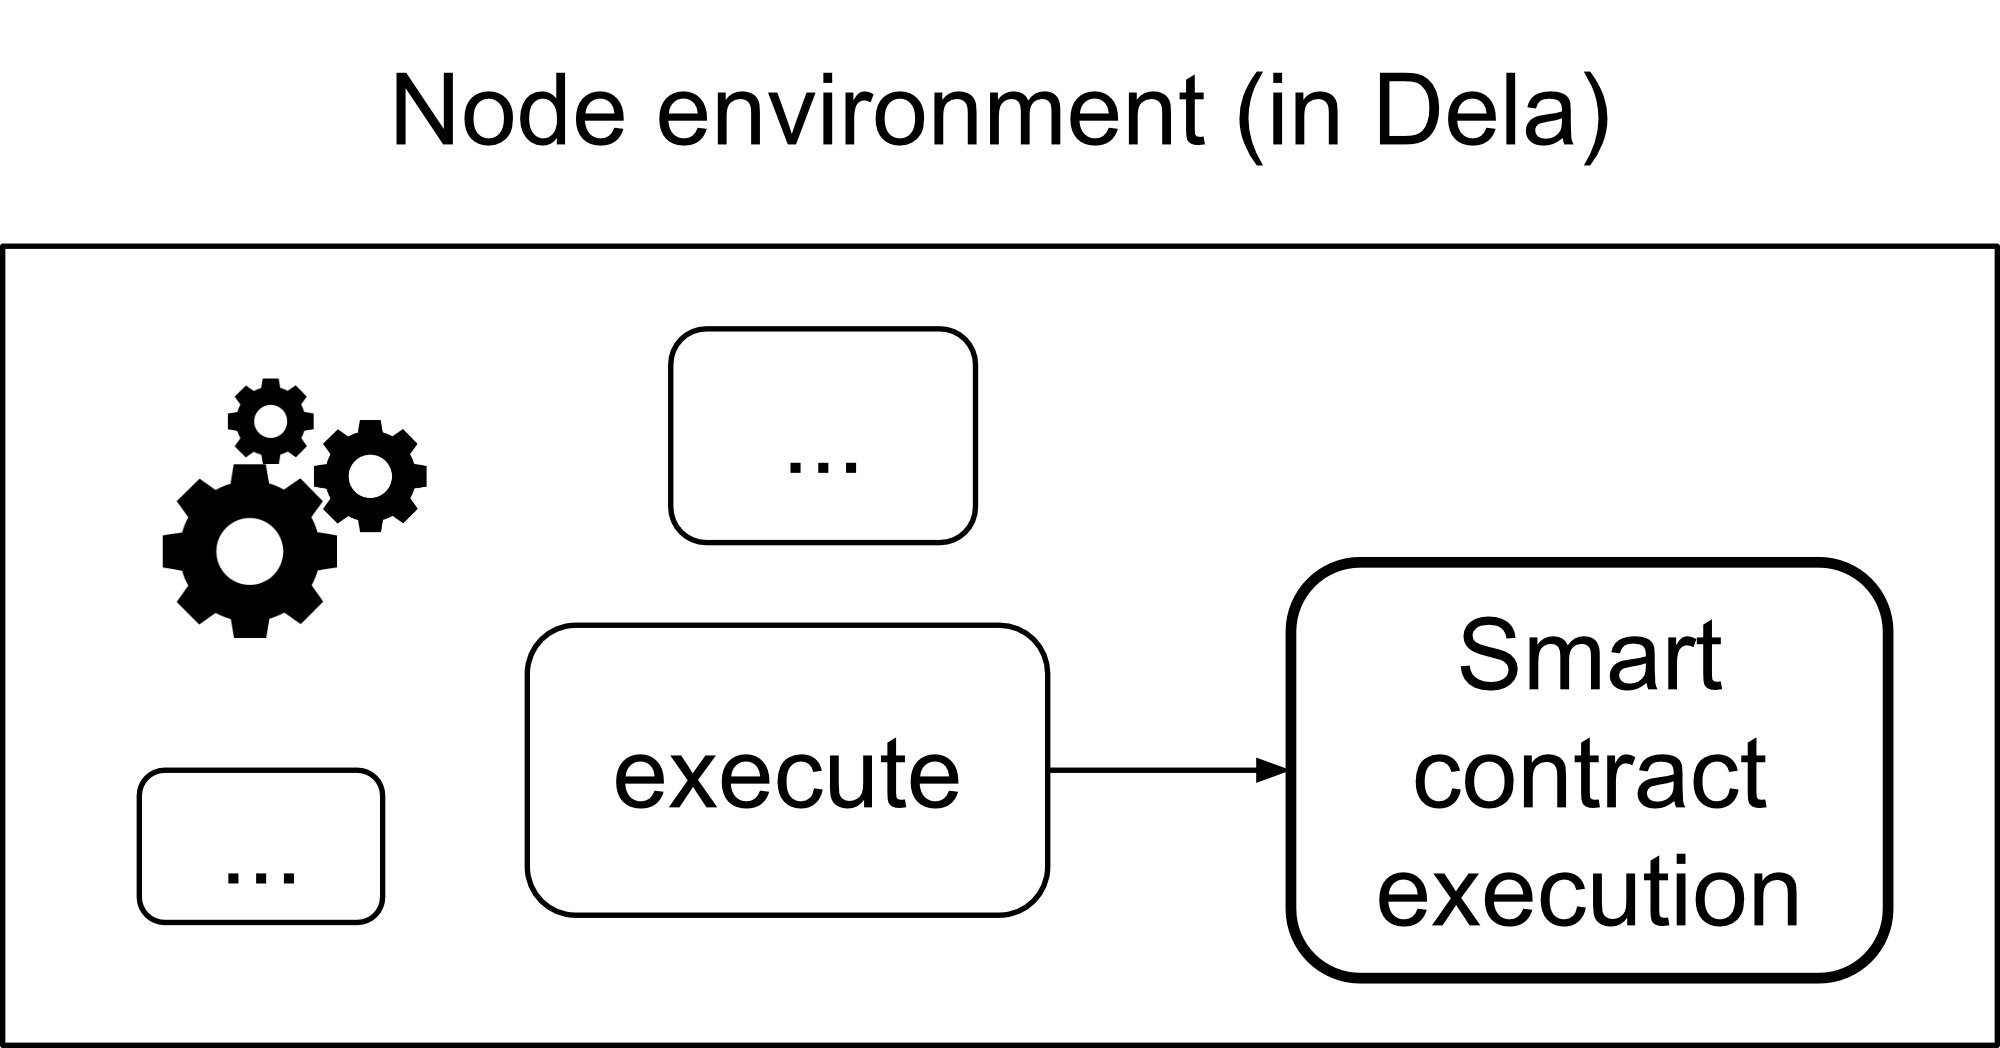
\includegraphics[width=12cm]{wasm1.png}
  \caption{Native smart contracts execution environment.}
\end{figure}


As shown in figure 1, the standard way of executing a smart contract in DELA is inside of a node's environment, which we call ``native'' execution. While this method is very intuitive and efficient, it has two main limitations. The first one is that adding, removing or modifying a smart contract requires re-compiling the entirety of the environment, which is highly unpractical in a realistic blockchain scenario where such changes are frequent. The second is that smart contracts are required to be pre-compiled for the environment running the ledger and must thus be written in the same language, which is Go in this case.

\begin{figure}[htbp]
 \centering
  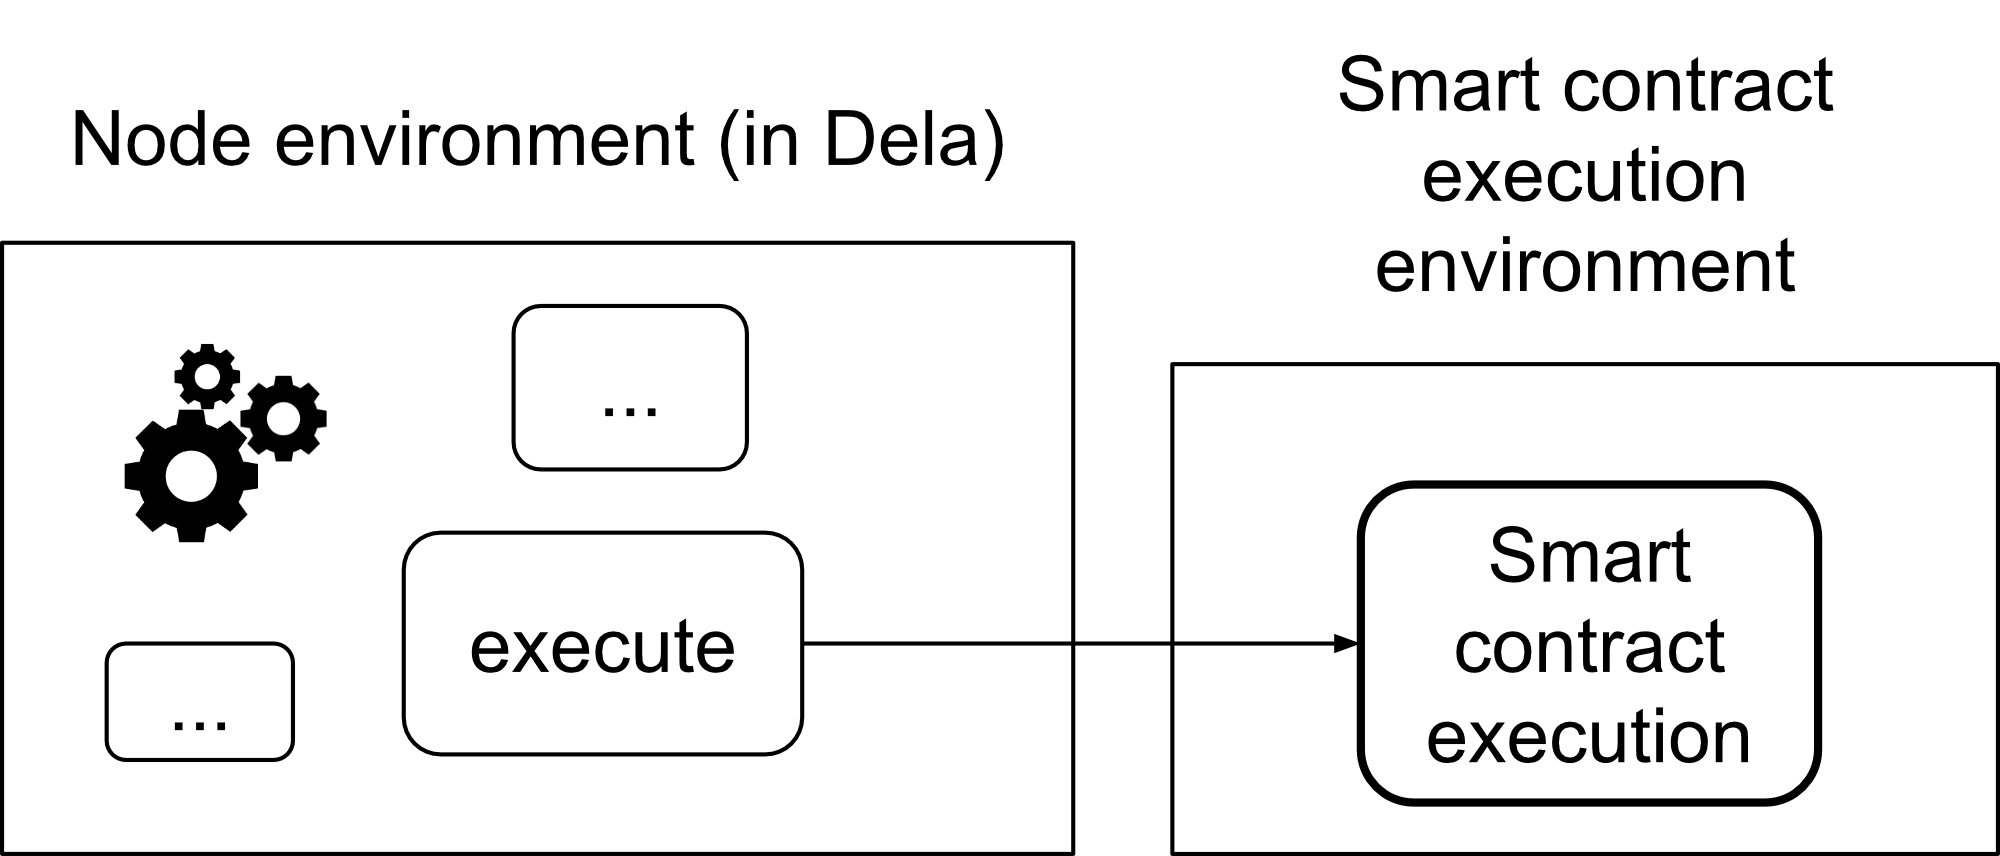
\includegraphics[width=12cm]{wasm2.png}
  \caption{Decoupled smart contracts execution environment.}
\end{figure}

To circumvent the first limitation, the obvious solution is to decouple the smart contract execution environment from the node's environment, as illustrated in figure 2. Any modification on the smart contracts would only require recompiling the smaller, decoupled environment which opens up the possibility of loading and unloading smart contracts dynamically without interrupting the main DELA environment. With this decoupled environment, smart contracts must not necessarily be written in Go, which somewhat takes care of the second limitation. However, supporting multiple languages efficiently is not straightforward and requires something else, which is when WebAssembly comes into the picture.

WebAssembly (WASM) is an open standard that defines a binary format which can obtained from higher level compatible languages, which we call ``source languages'' in this report. As its name implies, it is made up of low level ``Assembly-like'' instructions which can thus be run on a wide range of machines very efficiently. The WASM code is executed in a sandboxed environment. This added flexibility, its host independence and low performance penalty make it an ideal candidate for a smart-contract runtime used by many nodes trying to reach a consensus. Ethereum's proposed redesign of their execution layer using WASM further indicates that there is great potential for the technology in the blockchain field. 

\subsection{Goals}
\label{Goals}

\begin{enumerate} 

\itemsep0em

 \item Implementation of a fully functional execution module that uses WASM
 \item Simultaneous support of multiple smart contracts written in different languages
 \item Justification of configuration choices and the selection of compatible languages
 \item Performance comparisons
 \item Determinism analysis
 \item Testing comparable to the native module

\end{enumerate} 
\newpage

\section{Design}

\subsection{General Configuration}
The most important design decision during the project was selecting the ``kind'' of environment that should be implemented. WebAssembly was introduced in 2017 and its initial aim was to enable high performance web-browser applications with the help of a JavaScript API. Over time however, WASM started seeing use outside of browsers because of its many advantages, especially its near-native performance and consistent execution across different hardwares. As a result, three options were identified and considered : a web browser application, a web server and a unix daemon.

The first factor that was taken into account was the general lack of resources on WASM, which is severely exacerbated when the environment is not browser-based. Additionally, when dealing both with a non-browser solution as well as unusual source languages like Go, information about the specific interactions becomes virtually nonexistent. The daemon would have communicated with the DELA framework using unix sockets and would have used a runtime like Wasmer \cite{wasmer}, Wasmtime \cite{wasmtime} or WAVM \cite{wavm}, but was quickly deemed to be the riskiest option. Not only was it the least documented kind of environment and the most different from the standard browser solution, it was also identified that those non-web environments were transitioning to the Web Assembly Interface (WASI) \cite{wasi}\cite{announcingwasi}.

As a response to the aforementioned attempts to use WASM outside of web-browsers, WASI was introduced in 2019 to achieve standardisation and extend WASM to the OS level. The fact that it was newer and less mature than ``standard WASM'' further increased risks. Additionally, many languages such as Go do not yet support compilation into WASM binaries which are compatible with this interface. The transition also meant that almost all up-to-date information about non-web solutions were about using WASI.

The aforementioned points about the lack of resources and WASI not only apply to a unix daemon solution but also to a Node.js server-based solution communicating over HTTP, though less severely. While Node.js does expect its users to use its WASI API, it supports a limited portion of the standard WASM JavaScript API. However, there was no evidence that Node.js could handle Go's unusual WASM implementation in this specific context (which is further discussed in Part 3.2) and early tries to make it work failed.

Even though a web-browser application functionally makes less sense than the other options since the DELA framework would interact with it and not a human using a browser, it was thus the chosen solution during the early stages of the project and a working implementation was possible thanks to sufficient resources. However, its communication with DELA was initially simplified and it was identified that it would become very problematic as the environment would grow in complexity, since such a browser-based solution cannot easily and efficiently communicate with the framework. This prompted a second round of tries to make a Node.js solution work despite the limitations and the lack of information on unusual interactions.

Luckily, this second round was successful which was the best case scenario : a working Node.js solution which uses the Javascript ``standard WAS'' API and not the Node.js WASI API provides the best of both worlds for the project. Intentionally ignoring the WASI API limits risks as it is still experimental and enables the handling of smart contracts written in a wider range of languages. At the same time, using an HTTP server instead of a browser application provides an undeniably superior communication with the DELA framework. While the interaction with WASM binaries is not done with the intended Node.js API, this is the superior configuration for the project's specific needs at the present time ; there are currently no concrete time estimates on WASI support for multiple languages and on a stable release of the Node.js WASI API.


\subsection{Supported Languages}

Similarly to the freedom on the general configuration of the environment, the choice of which smart contract languages to support was free and part of the project.

Language compatibilities that were guaranteed to be worth prioritising are C and C++, since they were the two intended source languages when WebAssembly was introduced, before other languages added WASM compatibility as well. The target binaries are obtained from both languages with Emscripten \cite{emscripten}, a compiler toolchain which uses LLVM \cite{llvm}. The quality of the source language to WASM translation with Emscripten and the performance of the resulting binaries are considered to be state of the art in the world of WASM compatible languages, which made the environment support of the two languages even more indispensable since we are interested in comparing performance with native executions of smart contracts. Another obvious advantage is their extreme prevalence and that their simultaneous support incurs negligible additional work.

The other language which is supported is Go, which was chosen for many reasons. The first is that comparisons between the native and WASM executions can become more interesting when the exact same smart contract is compared in both cases, which is only possible if the native language is supported by the WASM environment. This can provide a precise comparison on the performance penalty caused by WASM and the communication with DELA, since external differences caused by differences in languages are removed. Another advantage is that Go is frequently used by the DEDIS lab, which means that its support could be very convenient in the future.

Something that was not known when choosing Go was a fundamental difference compared to other languages : C and C++ for example treat WASM as a library, while Go treats it as an application. This results in profound differences that requires the binaries to be treated very differently depending on the source language, even after the WASM compilation has been done. This caused many additional difficulties which are discussed in part 3 and a lot of the work done to support Go could not be reused to support C/C++. Even though this had a negative impact on productivity, this makes the addition of Go way more interesting than another language whose WASM support is similar to C/C++. Additionally, this allows interesting performance comparisons between what is considered the state of the art WASM support and a more subpar one in the case of Go. Since the project also mostly acts as an exploratory experiment, it is also good to prove that this kind of solution can handle less common languages with poorer WASM support.

Another language which was a strong candidate is Rust, which is commonly considered to have the second best WASM support after C/C++ and whose binaries are similarly obtained from Emscripten. It it not currently supported by the environment because other goals were judged more important than adding another language whose support is similar to two supported languages when the ability of the environment to handle different languages simultaneously was already demonstrated. However, its inclusion could be a worthy time investment in the future and should be straightforward considering the similarity of the process to the inclusion of C/C++.


\section{Implementation}

\subsection{WebAssembly Compilation}

In this project, the compilation of smart contracts to WASM must be done manually for each smart contract and the resulting binaries must be added to the environment before it is launched. Because of the aforementioned difference in the way Go and C/C++ treat WASM, the compilation process varies depending on the source language. Let us start by explaining the process for C/C++ since it is the standard.

A C/C++ smart contract must necessarily import the ``emscripten.h'' header file and can specify which functions to export, so that such functions can then directly be called from JavaScript in the server. The compilation is done with Emscripten, creating both the binary WASM file as well as a JavaScript file which will simplify the environment setup. Every necessary source and header files must be specified to Emscripten, which is important when entire libraries are imported by the smart contract. Emscripten can efficiently optimise the resulting binary file by stripping away code of libraries which is never used. Libraries which must usually be built with tools such as CMake must be built with Emscripten instead.

Unfortunately, this process proved to be extremely finicky in practice and would often fail for unintuitive or unclear reasons when large libraries where imported by the smart contract. This required manual changes which vastly differed for each library. Problems could arise both when building the required libraries with Emscripten and during the final compilation process. In the worst cases, the errors were devoid of sense and needed to be inelegantly avoided, for example by including parts of the problematic library directly inside of the smart contract. Personal experiments also indicated that these difficulties may vary depending on the hardware, which further complicates the process.

Let us now cover the process when the source language is Go. The smart contract must necessarily import the experimental ``syscall/js'' package to communicate with JavaScript. Compiling to WASM is natively supported but is only possible for ``main'' functions unlike in C/C++. For this reason, it is necessary to set the smart contract function to the global JavaScript object inside of the main Go function, which allows it to be called directly from JavaScript as is the case for C/C++. Unlike the process with Emscripten, the Go to WASM compilation succeeded without issues most of the time. However, it always generates very large binaries of several megabytes and is highly dependent on the imported packages, unlike Emscripten which prunes unused code more efficiently. Using TinyGo \cite{tinygo} (which is also uses LLVM) can reduce this size but does not support every language feature, which may be an issue for some smart contracts.

The original smart contracts written in their source language are included along their corresponding WASM binary for readability and to allow users to do the compilation themselves if desired. The necessary commands are included as comments in every smart contract, which is particularly useful for C/C++ smart contracts as the commands are particularly long and complex.

\subsection{Environment Setup}

The environment is launched with one simple Node.js command and must automatically set up the smart contracts from the included WASM binaries as well as the HTTP communication with the framework before any execution request is sent from DELA. To improve the global execution time, the environment mus obviously do as much work as possible before it receives its first request.

Instantiating the C/C++ is straightforward : the JavaScript modules created with Emscripten mentioned in the previous subsection are first included, which then allows each function to be instantiated. The Go instantiation proved way more troublesome since only some parts of the JavaScript WASM API work on Node.js and that Go has an unusual WASM support since WASM is treated as an application instead of a library. A very specific way to instantiate Go smart contracts proved to be working when recommended methods previously failed on Node.js. 

Unlike C/C++ which can efficiently and durably export functions to the environment, Go only sets them in the global JavaScript object as long as its main function is running. This requires artificially keeping the program open indefinitely so that the environment can use the smart contract function at any time while specifying arguments. In our case, this is simply achieved in each Go program by waiting to receive a value which never arrives from a channel in main() after having set the useful smart contract function to the global JavaScript object. It is not possible to use a WASM binary where the smart-contract operations are contained in the Go program's main function : such a binary would be run in its entirety multiple times without needing to keep it indefinitely running but is not feasible simply because a main function does not take arguments nor does it return anything. It is thus necessary to export non-main functions to the the environment in this odd way if any sort of communication between the environment and the smart contract is required.

An optional step that the environment can take during its setup is to ``warm up'' each smart contract by launching each exported WASM function with meaningless but realistic arguments, while ignoring the resulting output since it is meaningless as well. This was found to have a positive impact on the performance of the following first real execution of the corresponding smart contract when requested by DELA, especially for C/C++ ones. However, this does not benefit any subsequent execution and comes with the cost of significantly increasing the setup time, which is obviously dependent on the number of smart contracts the environment supports. Because this step is inelegant and its limited benefits are not necessarily needed, it is disabled by default.

An intentionally simple Rest API is then launched and the server listens to a specific port on the local host which is arbitrarily chosen and known by DELA.
 
\subsection{Smart Contract Execution}

The requests to execute a smart contract with specific arguments that the environment receives always have a JSON structure, which contains both the smart contract name as well as the arguments. When such a request is received, the environment reads two fields of the received JSON to get the smart contract's unique name and its source language. The latter is specified because multiple versions of a same smart contract could be instantiated and available from different source languages. Each WASM binary must be placed in the right folder specifying the source language, so that multiple binaries of the same name but obtained from different source languages can be supported simultaneously. 

The environment can then call the right exported method with the entire JSON as an input in string format. C/C++ executions require slightly more work than Go's because the string needs to be allocated to the function's instance, then freed once the execution's result is stored. The result of the execution must also have a JSON structure, which contains information about the success of the execution, writes to the ledger's storage and potential errors.

Because of this design, each smart contract must handle JSON structures in the original program written in the source language before getting compiled to WASM. This means that smart contracts which are already written must be slightly adapted before being compatible with this specific environment. However, this does not require any deep redesign since the required additions only affect the smart contract's input and output. If the JSON structure handling is added at the start and end of the function, it becomes compatible with the environment without any need to change the smart contract's actual process and can be compiled to WASM.

\subsection{Communication with DELA}

\begin{figure}[htbp]
 \centering
  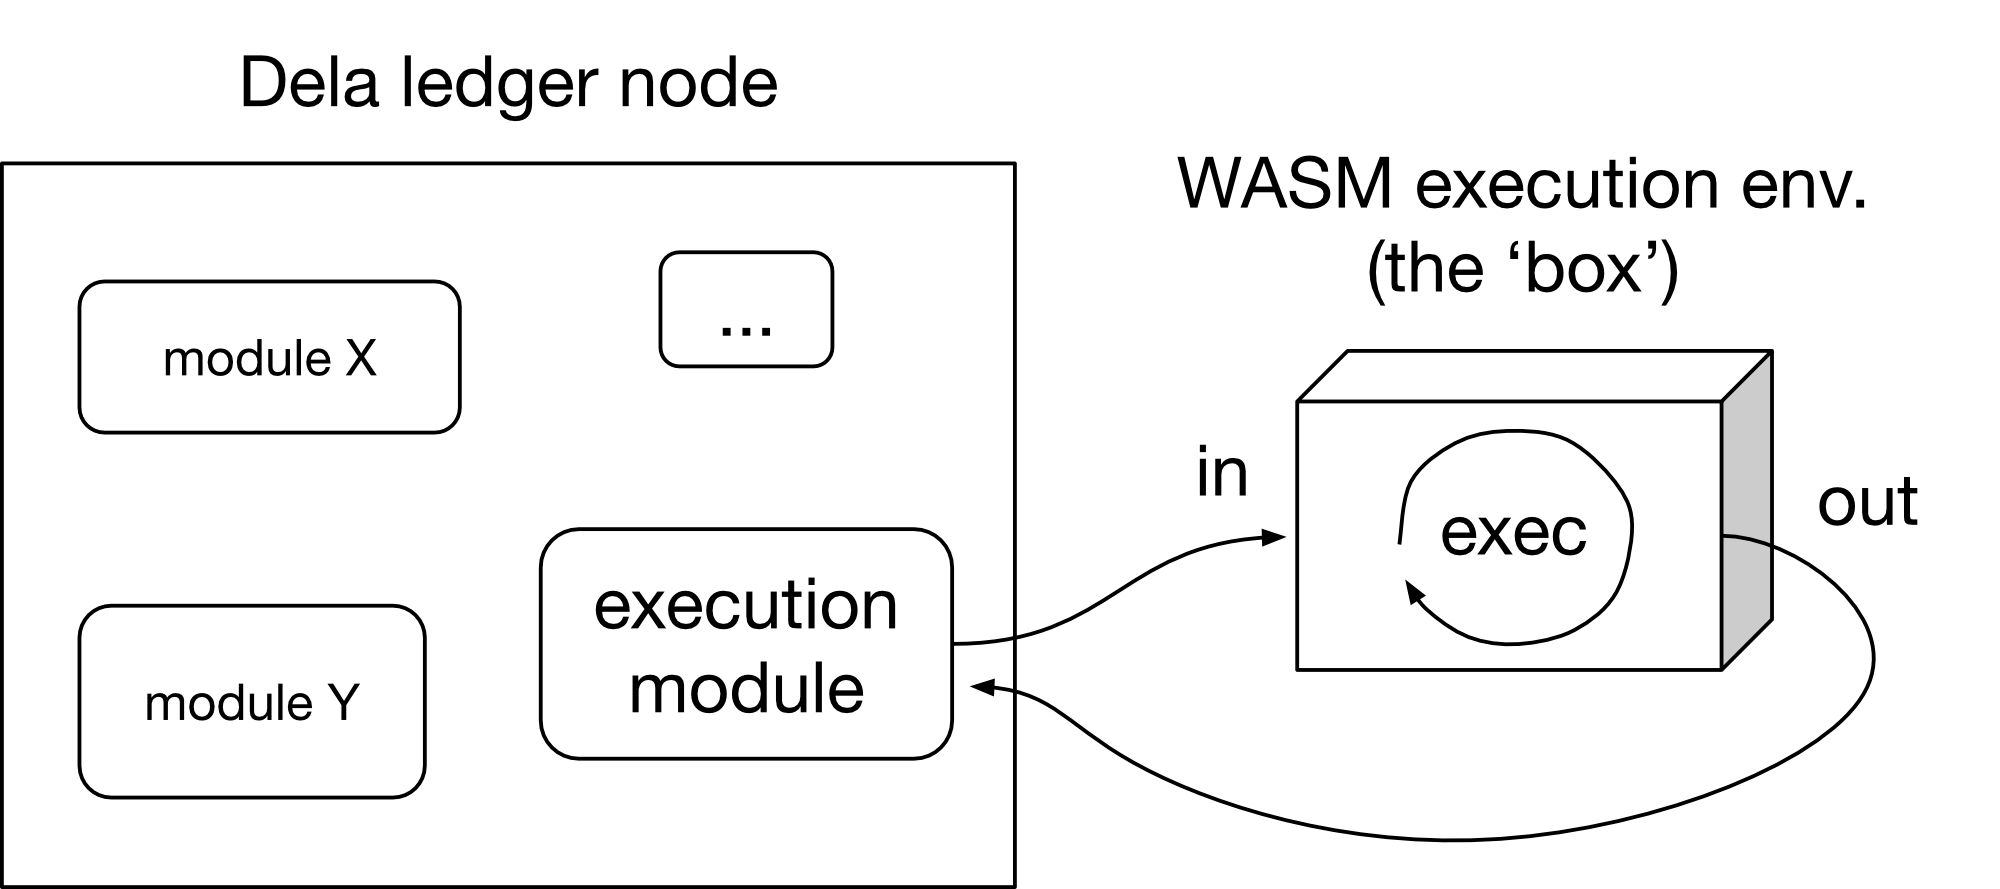
\includegraphics[width=12cm]{wasm3.png}
  \caption{Communication between the DELA execution module and the environment.}
\end{figure}

Since the communication is one to one (each node from the DELA ledger has its own WASM environment) there was no need for a complex Rest API using a web application framework. For this reason, the HTTP server was intentionally simple and built using Node.js's ``http'' module only. The aforementioned use of JSON structures was chosen because of its flexibility while being able to be sent over HTTP during both transmissions. This sometimes led to necessary translations between bytes and strings using Base64 encoding both inside of the DELA framework and inside of smart contracts since JSON does not support raw bytes. The communication process is again intentionally simple : both data transfers seen in figure 3 only consist of one JSON file. Each one contains every information, which can easily be retrieved since the keys are agreed upon by DELA and the environment.

Outside of the transaction itself, some parts of the ledger's storage must also be sent over to the environment because smart contracts may need to read or write content on it such as its state. However, the parts of the storage which are necessary change depending on the smart contract. Sending the entirety of the storage would be the easiest solution but would be very inefficient. As DELA matures and transactions become more realistic and complex, a system needs to be implemented which sends only the essential parts of the storage. The solution should be to create a map accessible by DELA's execution module which specifies which parts of the storage must be included in the JSON to be sent over to the environment depending on the smart contract name, which would be the keys of the map. Note that the source language of the smart contract does not affect which parts of the storage are required. This would be the easiest and quickest way for the module to obtain the subset of the storage to include in the JSON with the unique smart contract name.

Errors are handled and relayed across the different parts so that the DELA can directly read eventual errors. However, only ``honest'' mistakes are assumed since the environment is located on the same machine as the DELA node : we do not consider either to be a potentially harmful to the other. For example, we do not expect the node to divert from protocol and send unusual data to the environment in an attempt to shut it down since it has no reason to do so. Even a hostile node would gain no benefit by making its own WASM environment behave in an unusual manner : the environment is nothing more than a tool serving the node.

\section{Results}

\subsection{Counter Increase}

\begin{figure}[H]
 \centering
  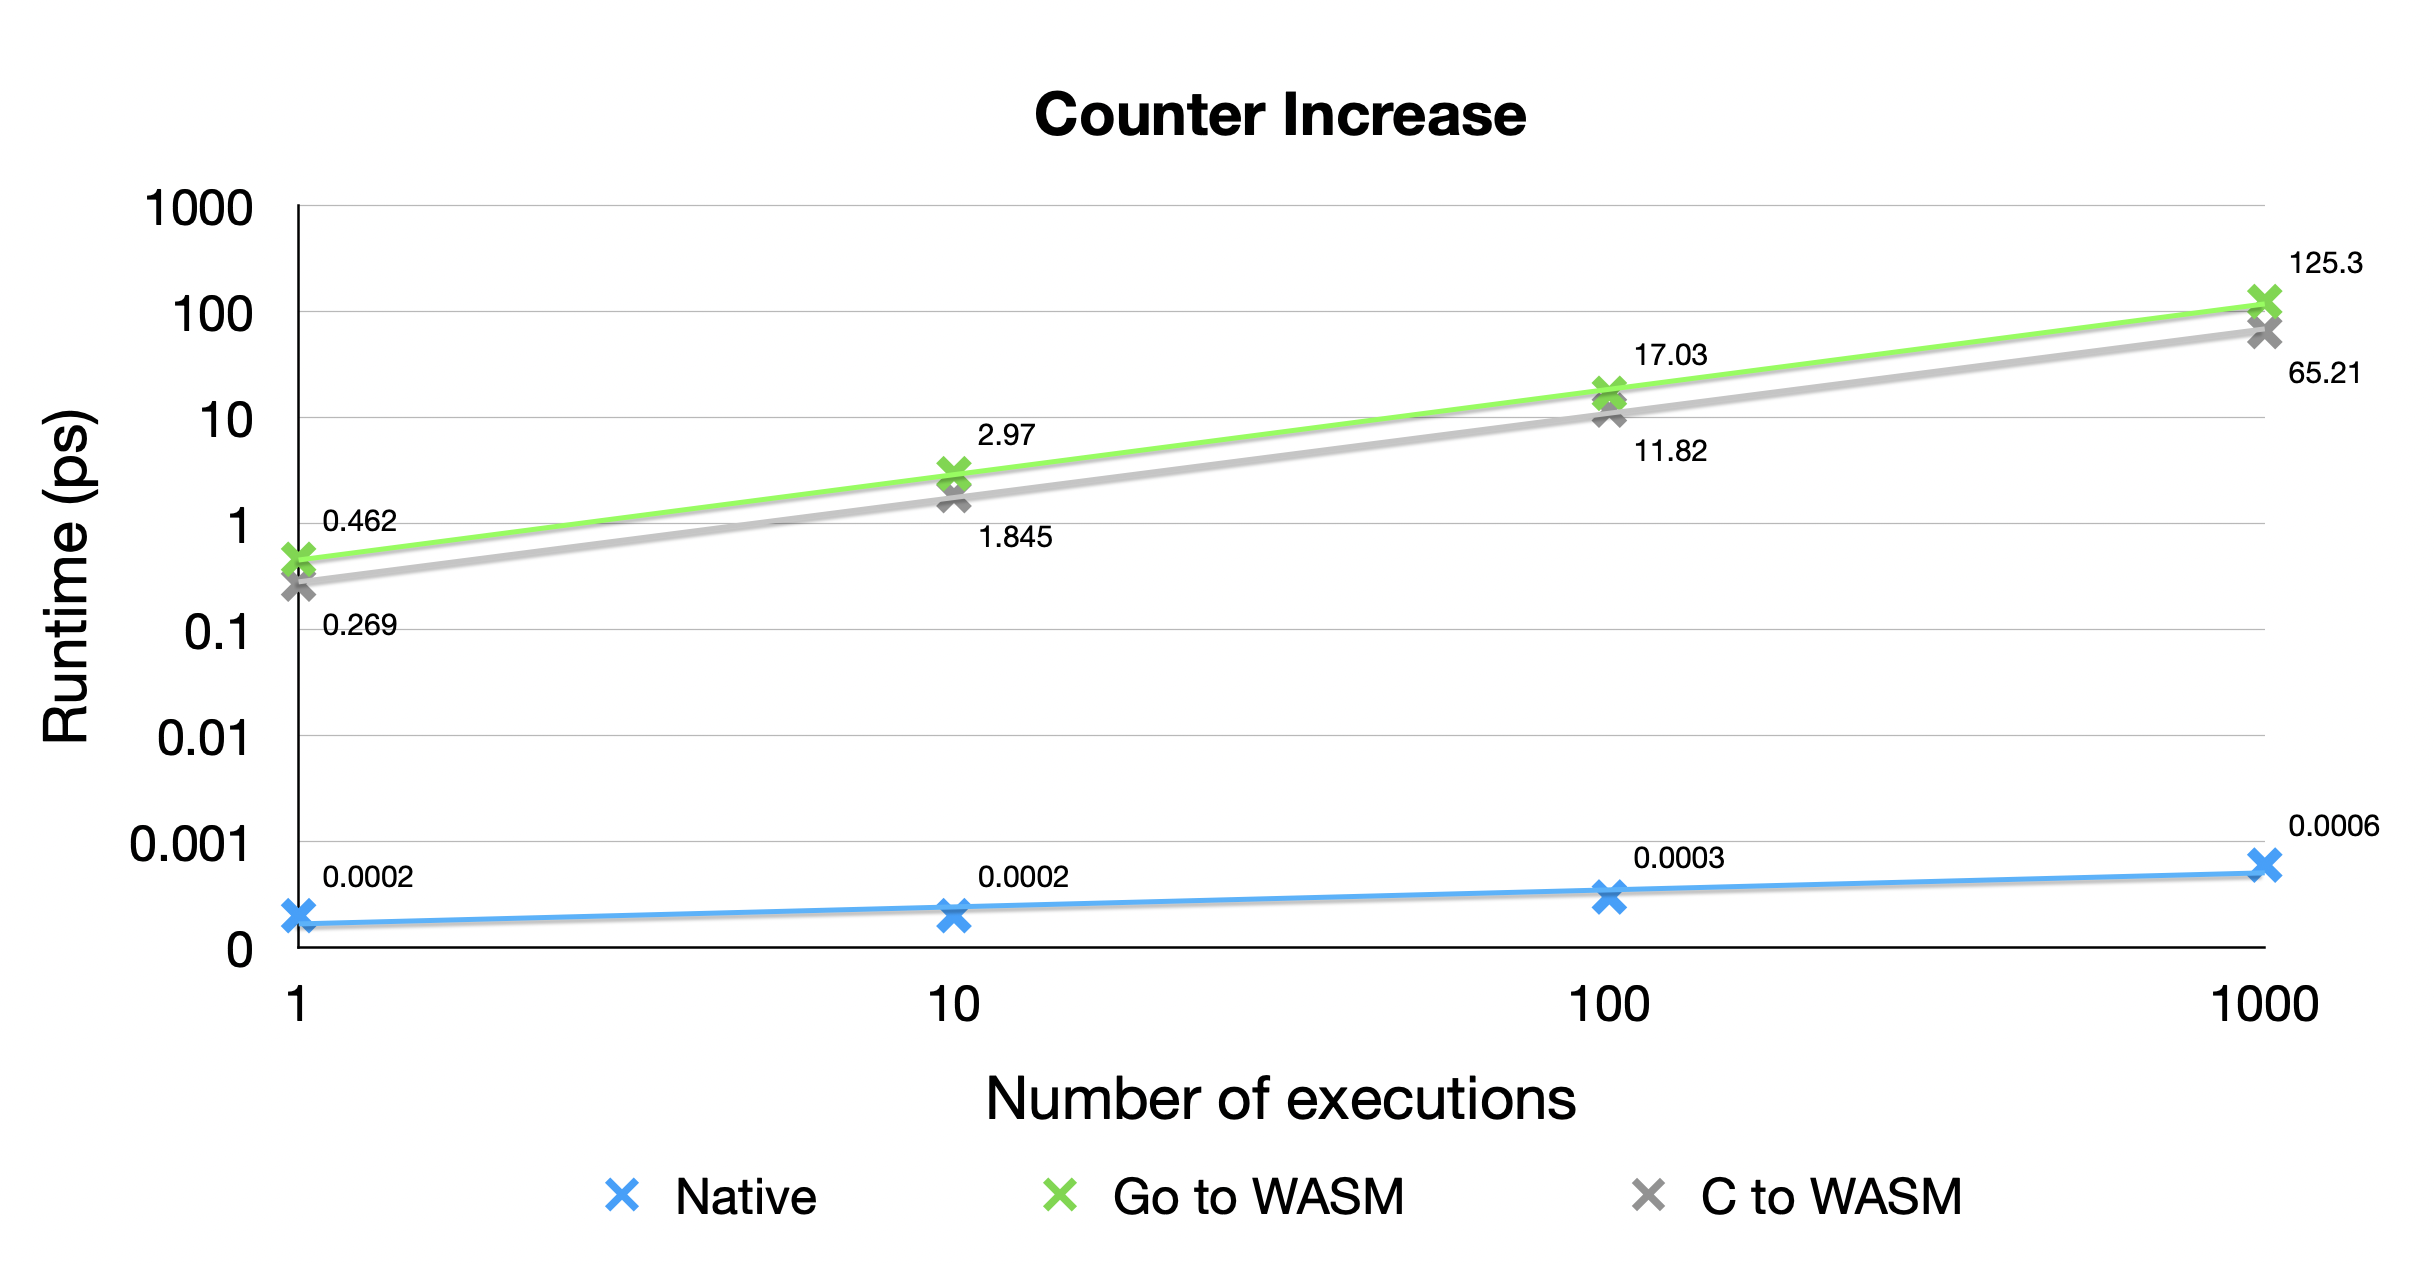
\includegraphics[width=14cm]{increase_counter.png}
\end{figure}



\subsection{Generator Multiplication}

\begin{figure}[H]
 \centering
  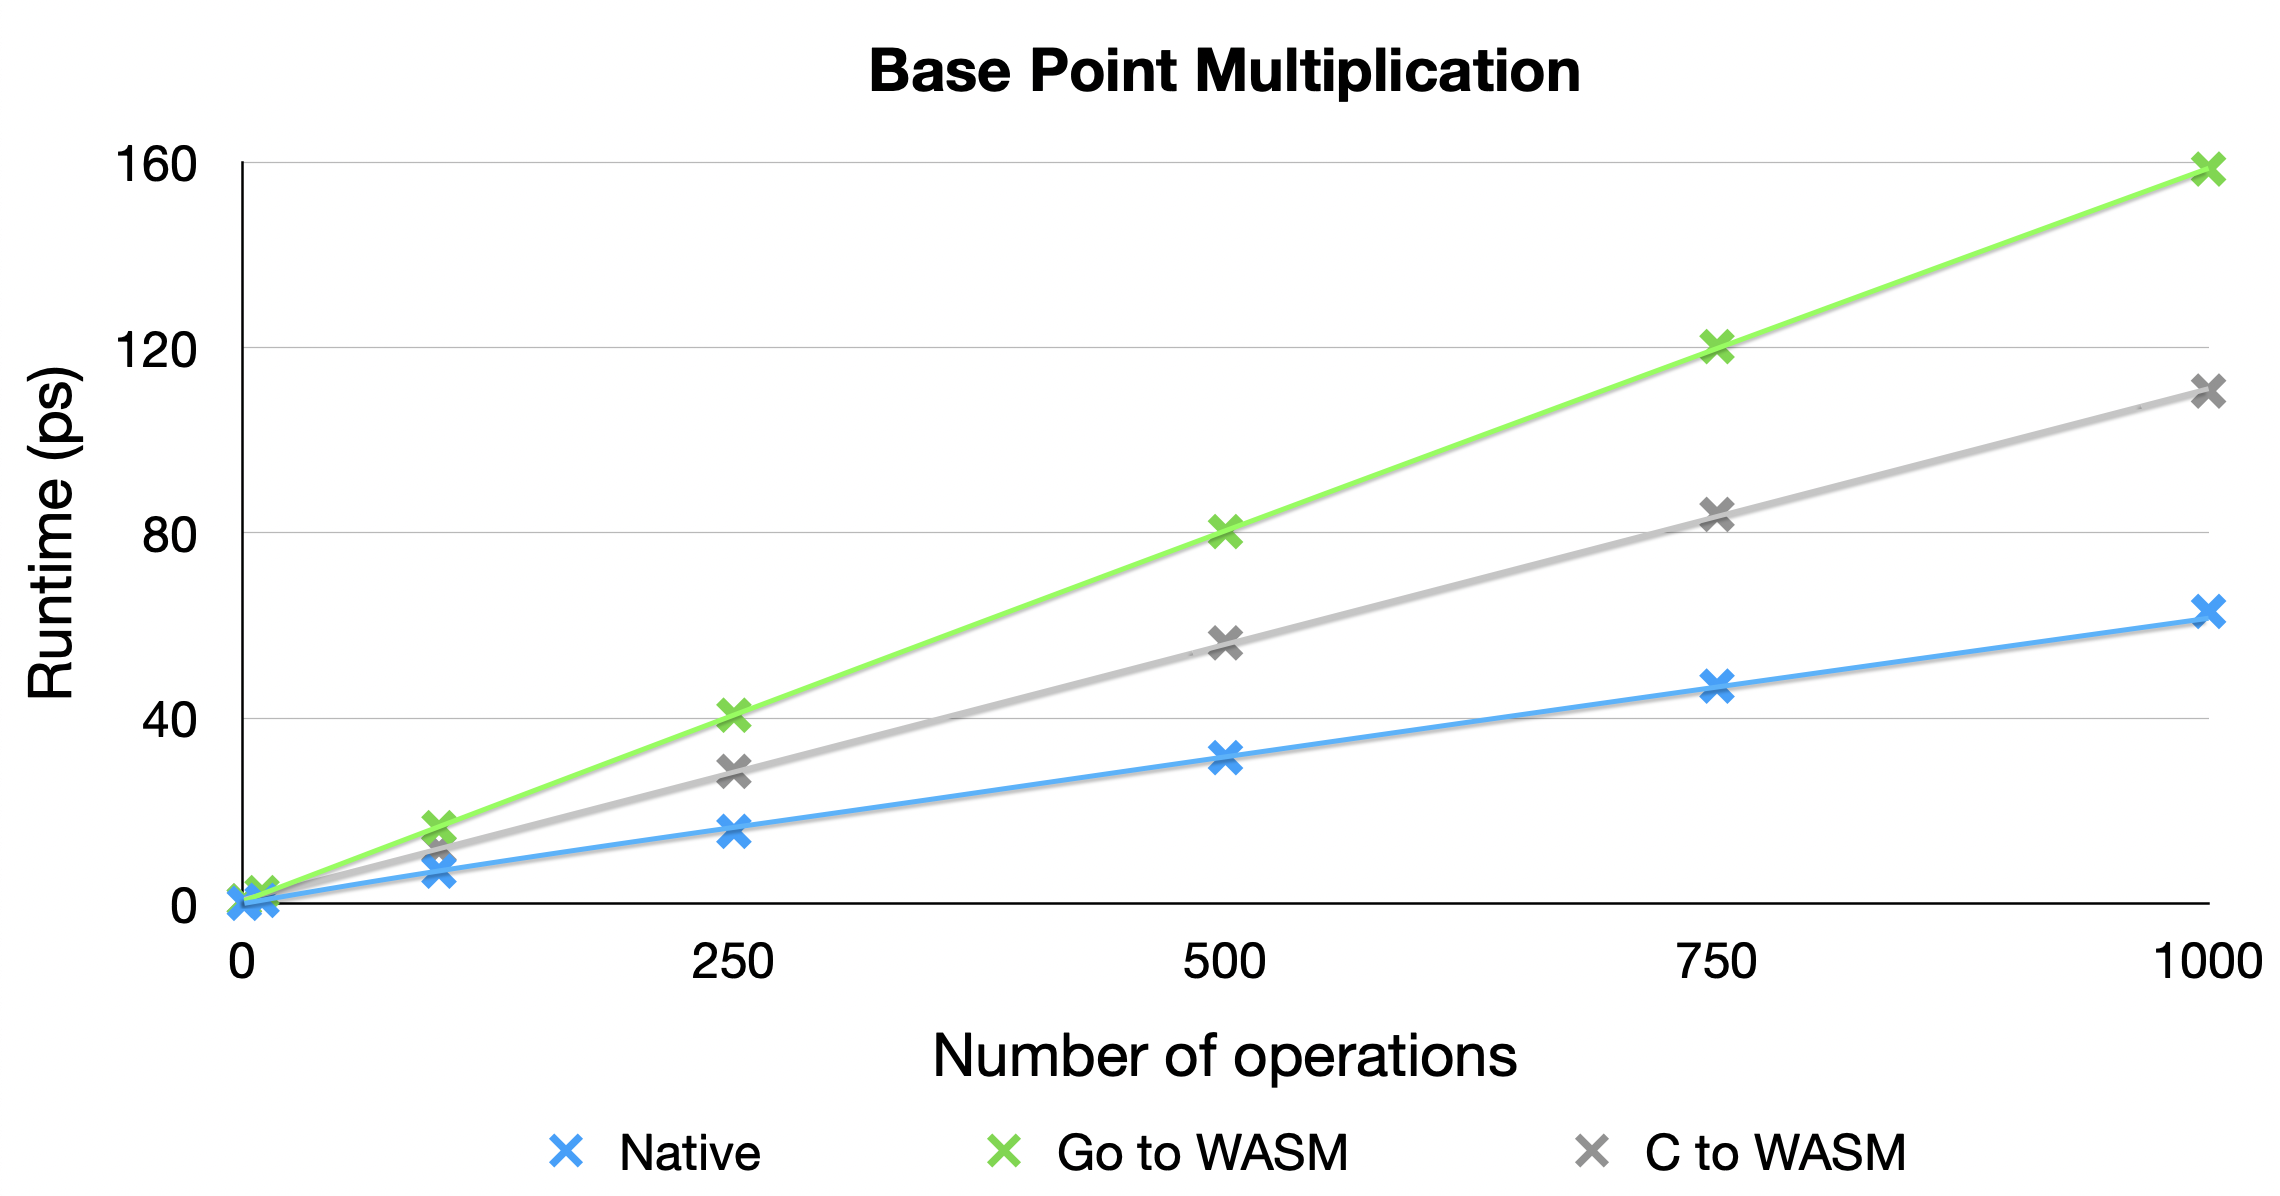
\includegraphics[width=14cm]{gen_mul.png}
\end{figure}


\subsection{Ed25519 Point Addition}

\begin{figure}[H]
 \centering
  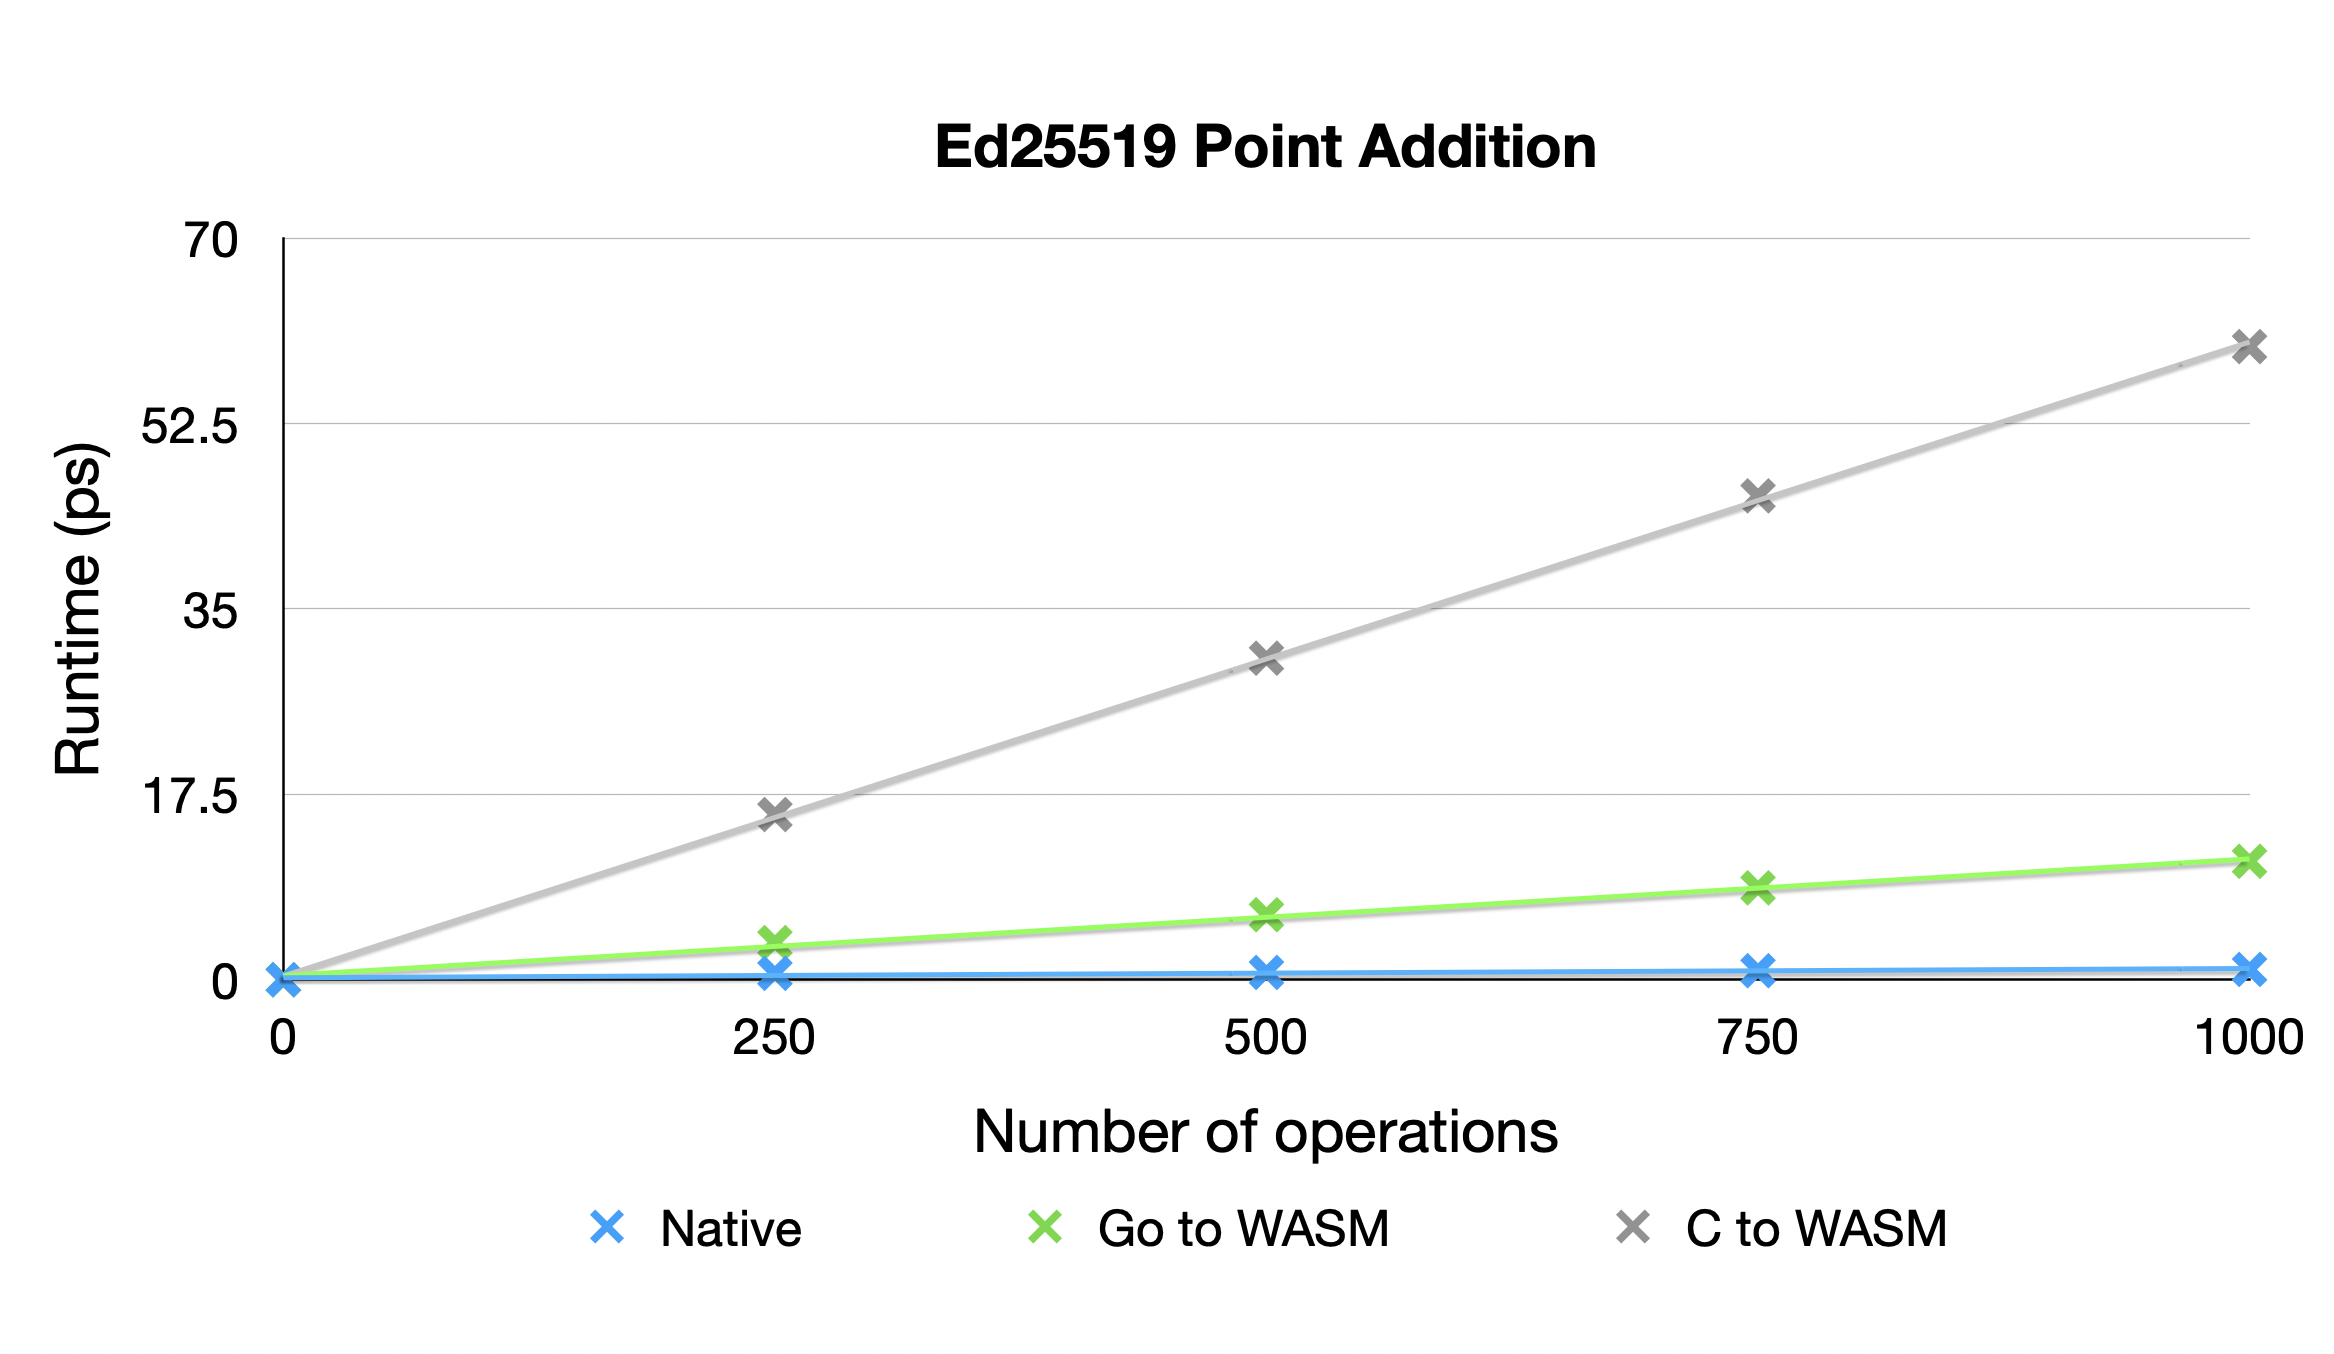
\includegraphics[width=14cm]{point_add.png}
\end{figure}



\subsection{Ed25519 Point Multiplication}

\begin{figure}[H]
 \centering
  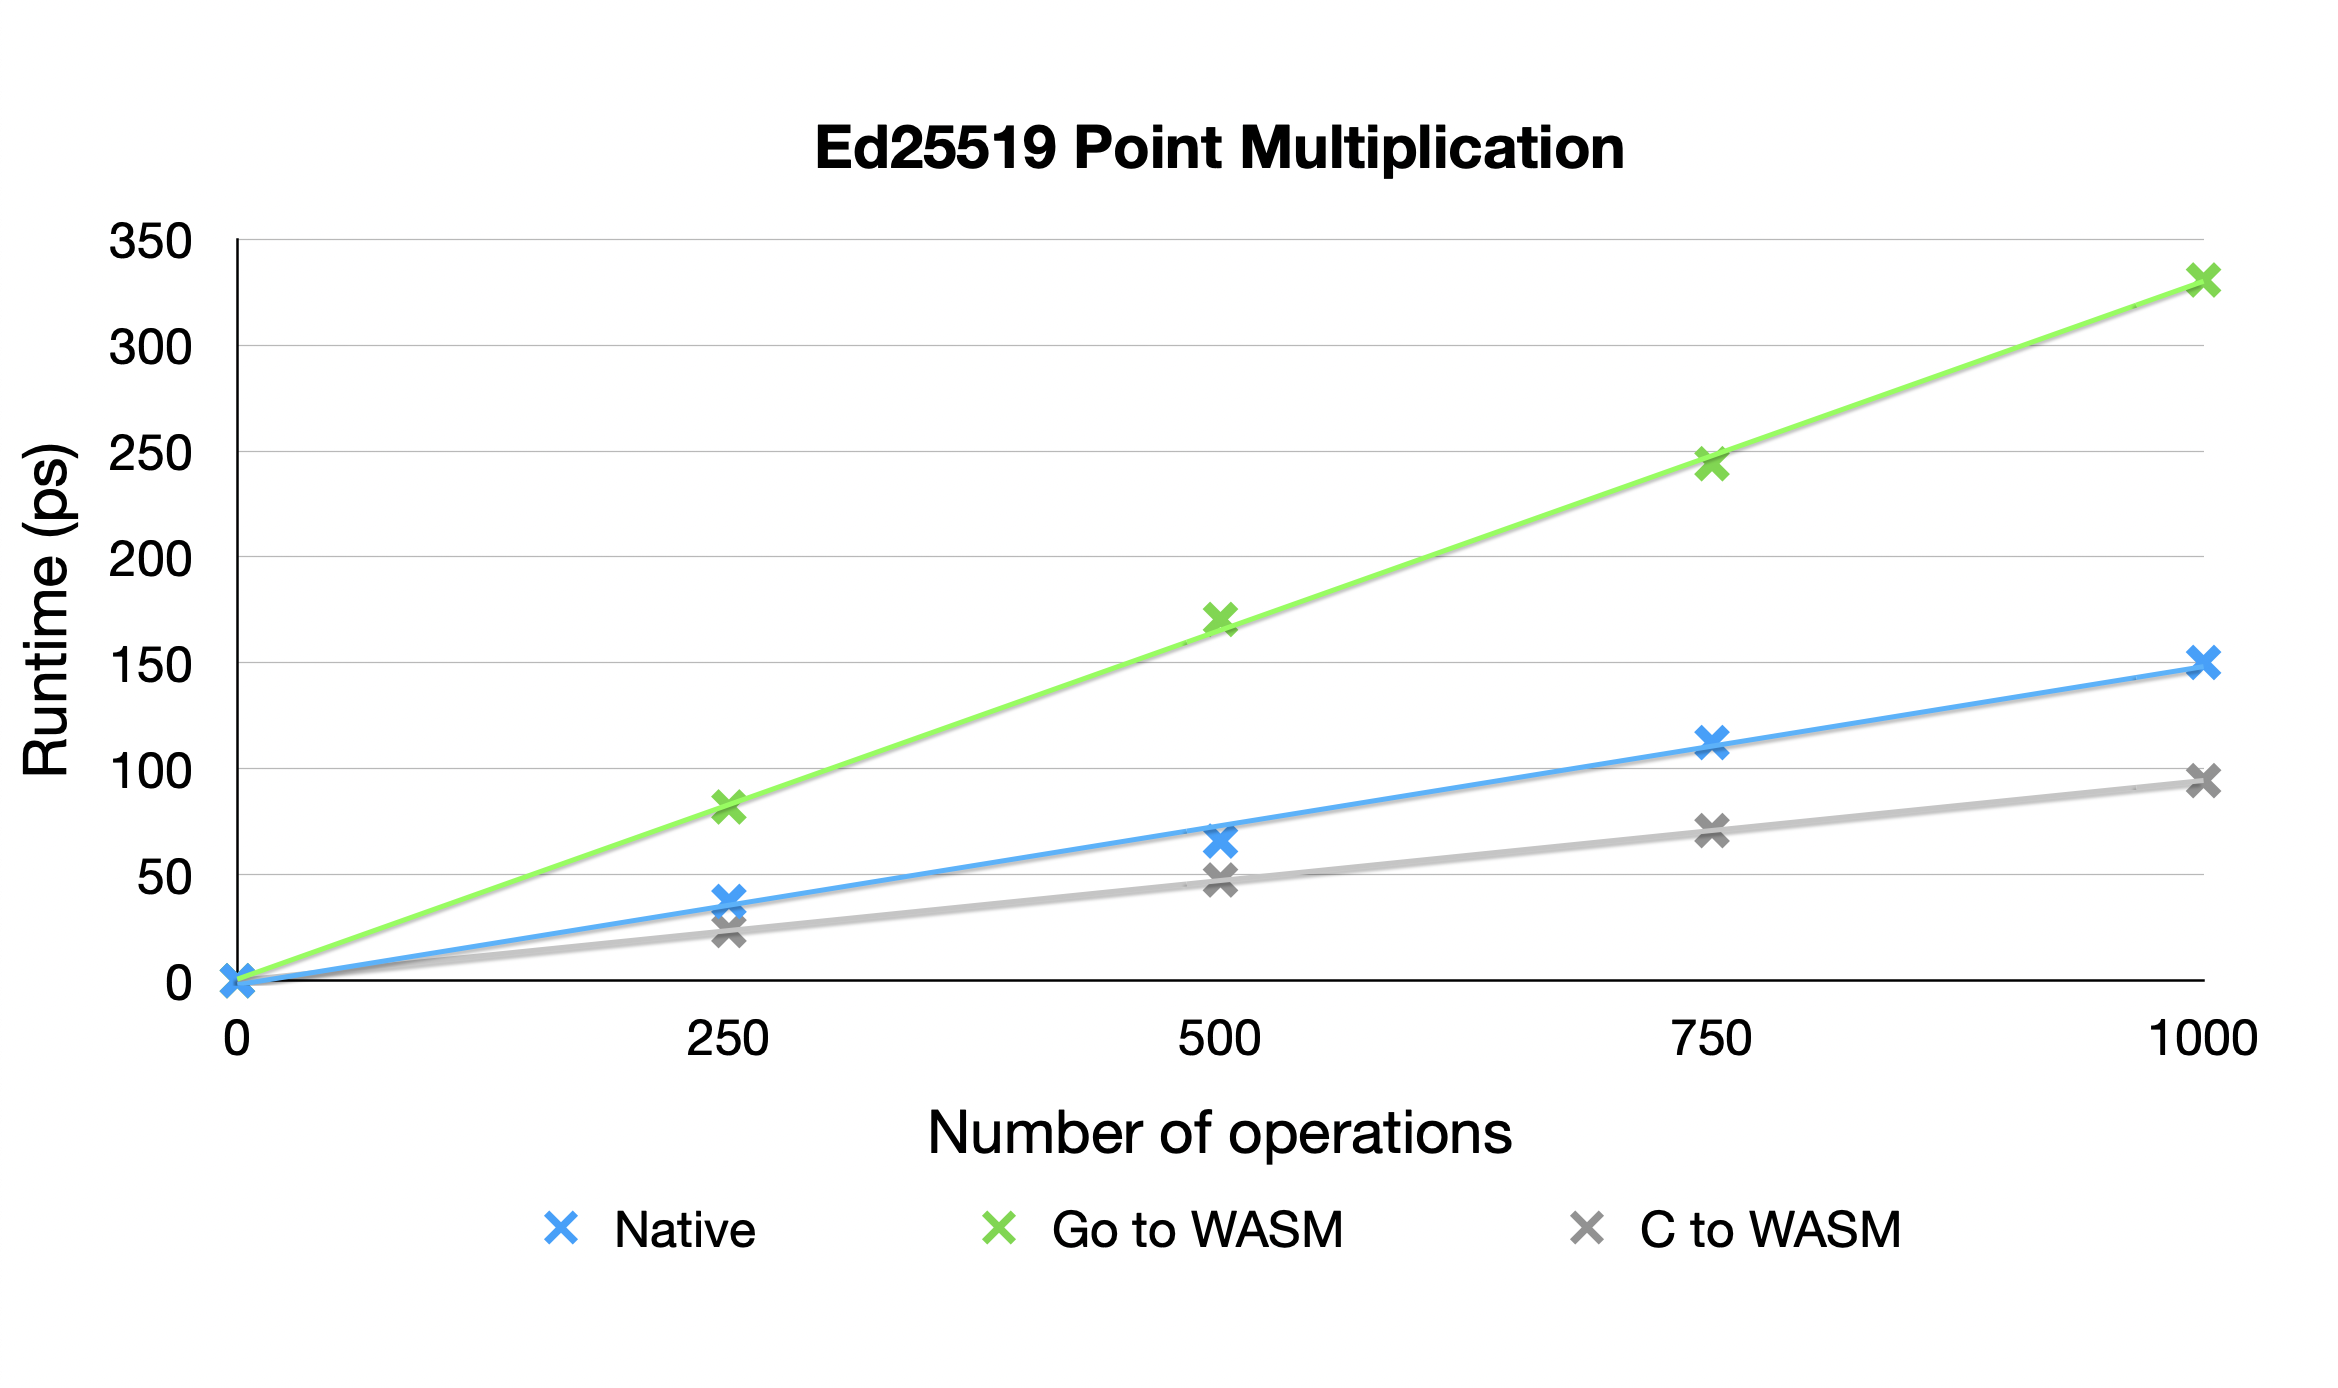
\includegraphics[width=14cm]{point_mul.png}
\end{figure}



\section{Discussion}

\subsection{Determinism}

\subsection{Automated Smart Contract Loading}


\section{Future Work}

\section{Conclusion}
\newpage
\section{Bibliography}
\bibliographystyle{unsrt}
\bibliography{biblio}
\end{document}
